\documentclass[12pt, a4paper]{article}

\usepackage[T1]{fontenc}
\usepackage[utf8]{inputenc}
\usepackage{mathpazo}
\usepackage{microtype}
\usepackage{amsmath, amssymb, amsthm}
\usepackage{mathtools}
\usepackage{geometry}
\geometry{a4paper, top=2.5cm, bottom=2.5cm, left=3cm, right=3cm}
\usepackage{setspace}
\onehalfspacing
\usepackage{titlesec}
\usepackage{hyperref}
\hypersetup{colorlinks=true, linkcolor=black, citecolor=black, urlcolor=black}
\usepackage{csquotes}
\usepackage{tikz}
\usetikzlibrary{shapes.geometric, arrows.meta, positioning, fit, calc}

% Hyperbionic emphasis operators — visual energy proportional to conceptual salience
% \hyperemph  = medium energy (e_i elevated, s_i > 0.7)
% \hyperstrong = high energy  (e_i maximal, s_i \approx 1)
% Applied only to invariant identities, ontological pivots, and structural definitions.
\newcommand{\hyperemph}[1]{\textbf{\large #1}}
\newcommand{\hyperstrong}[1]{\textbf{\Large #1}}

\titleformat{\section}{\large\bfseries}{}{0em}{}[\vspace{0.4em}\hrule\vspace{0.6em}]
\titleformat{\subsection}{\normalsize\bfseries\itshape}{}{0em}{}

\newtheorem{theorem}{Theorem}
\newtheorem{definition}{Definition}
\newtheorem{proposition}{Proposition}

\title{\textbf{Hyperbionic Reading:\\
A Visual Projection of Prosodic Parameter Space}}
\author{Flyxion\\
\small Independent Researcher}
\date{}

\begin{document}

\maketitle

\begin{abstract}
\noindent
Written language is a lossy projection of speech that preserves lexical structure while discarding prosody, timing, and spatial acoustics. This essay proposes Hyperbionic Reading as a formal system that restores these lost dimensions by embedding prosodic invariants directly into the visual properties of typography. We establish that acoustic analysis, modal resonance storage, and Hyperbionic rendering are not merely analogous but equivalent as parameterized projections of a shared invariant structure: the prosodic parameter vector extracted from a waveform by peak-derived measurement. This equivalence extends to higher-dimensional acoustic features---delay and reverberation---which admit precise typographic operators. The analysis is further extended into the temporal domain, where spoken words are treated not as static points in feature space but as trajectories through a modal lattice, yielding a wave-native architecture for speech recognition as trajectory resonance. The culminating claim is that marked-up text is not decorated language but a higher-dimensional prosodic encoding, and that Hyperbionic Reading is the visual projection of the same invariant structure that acoustic analysis measures and resonant memory stores.
\end{abstract}

\newpage

\section*{Orientation}

The following exposition develops the theoretical foundations of Hyperbionic Reading as a system for restoring prosodic structure to written language. The central claim is that prosody is not an ancillary feature of speech but a measurable, invariant structure that admits consistent representation across acoustic, geometric, and visual domains. This document should be read as the construction of a single invariant object viewed through multiple coordinate systems. The acoustic waveform, the modal lattice coordinate, and the Hyperbionic rendering are not independent representations but projections of a shared prosodic field. The purpose of the exposition is therefore not to introduce separate techniques but to show that these apparently distinct operations commute: measurement, storage, and rendering preserve the same structure under change of medium. Each section re-establishes the invariant before developing the next layer of the pipeline.

A note on presentation: the paper applies its own rendering operator to itself. Invariant identities, ontological pivots, and structural definitions are rendered at elevated visual energy (larger, bolder type), corresponding to high values of $e_i$ and $s_i$ in the Hyperbionic parameter space. This is not stylistic decoration but a proof of concept: the same emphasis logic that the theory describes is instantiated in the typography of the document.

\section{Introduction: Text as Lossy Projection}

When speech is transcribed into writing, the resulting symbol sequence preserves very little of the original signal. Lexical content survives---the identity of words, their grammatical arrangement---but the continuous structure that carries a large fraction of communicative meaning does not. Pitch contour, amplitude envelope, temporal rhythm, the degree of periodicity in voiced sounds, the spatial diffusion of reverberation: none of these are recoverable from a plain text string. The information they carry---emotional valence, prosodic emphasis, the speaker's certainty or hesitation, the acoustic properties of the environment---is simply absent.

This is not an incidental limitation of writing systems. It is a structural consequence of reducing a high-dimensional continuous signal to a sequence of discrete categorical tokens. The question this essay addresses is whether that reduction is necessary, or whether typography can be extended into a system that preserves prosodic structure by distributing it across the visual degrees of freedom that rendered text already possesses but does not exploit: size, weight, baseline position, spacing, rotation, opacity, blur, layering.

The answer developed here is that such an extension is not merely possible but formally well-defined. What is required is not an augmentation of text but a reconstruction of the signal pathway that was collapsed during transcription. This pathway consists of three operators: a measurement operator $\mathcal{M}$ that extracts prosodic invariants from sound, a storage operator $Q$ that preserves those invariants geometrically, and a rendering operator $R$ that re-expresses them in a visual medium. \hyperstrong{Hyperbionic Reading is not decorated text. It is a projection of prosodic signal into visual space.} The extension requires three things: a compact representation of the prosodic structure of an acoustic signal, an operator that maps that representation into visual parameters, and a notion of equivalence across the acoustic, stored, and visual forms of the same prosodic information. Each of these is developed in turn.

\section{The Prosodic Measurement Operator}

\noindent\textit{This section formalizes prosody as a measurable physical structure by identifying the minimal set of signal events from which invariant quantities can be extracted. The key move is to replace uniform sampling with event-based sampling: instead of analyzing every point in the waveform, the system tracks peaks, which concentrate the signal's energetic and temporal structure.}


Let $u(t)$ denote an acoustic waveform, a real-valued signal defined over a time interval $[0, T]$. A prosodic analysis of $u(t)$ extracts from it a finite-dimensional vector of physically interpretable invariants. The central object is the \emph{prosodic measurement operator}

\begin{equation}
\mathcal{M} : u(t) \mapsto \mathcal{M}(u) \in \mathbb{R}^n,
\label{eq:M}
\end{equation}

which maps a waveform to a coordinate in prosodic parameter space. This is not an embedding in the machine-learning sense: the components of $\mathcal{M}(u)$ are not learned abstractions but measured physical quantities, computable from the peak structure of the waveform.

For a concrete and sufficient instantiation, let $\{t_k\}_{k=1}^N$ denote the sequence of peak times in $u(t)$ and $\{a_k\}_{k=1}^N$ the corresponding peak amplitudes. Define the inter-peak intervals $\Delta t_k = t_k - t_{k-1}$, the period jitter values $j_p(k) = |\Delta t_k - \overline{\Delta t}| / \overline{\Delta t}$, and the amplitude jitter values $j_a(k) = |a_k - \bar{a}| / \bar{a}$, where overbars denote sample means. The measurement operator then returns the eight-dimensional vector

\begin{equation}
\mathcal{M}(u) =
\left(
\overline{j_p},\;
\sigma_{j_p},\;
\overline{j_a},\;
\sigma_{j_a},\;
h,\;
s,\;
\rho,\;
E
\right) \in \mathbb{R}^8,
\label{eq:Mvec}
\end{equation}

where $\overline{j_p}$ and $\sigma_{j_p}$ are the mean and standard deviation of period jitter, $\overline{j_a}$ and $\sigma_{j_a}$ are the mean and standard deviation of amplitude jitter, $h$ measures harmonic coherence (the degree of periodic regularity in the voiced signal), $s = (1 + \overline{j_p} + \overline{j_a})^{-1}$ is a salience index that varies inversely with total jitter, $\rho = N/T$ is peak density in events per second, and $E = N^{-1}\sum_k a_k^2$ is mean squared amplitude.

Several features of this definition deserve emphasis. The vector is low-dimensional relative to the signal itself---eight scalars from a waveform of potentially millions of samples---but each dimension is physically interpretable and stable under small perturbations of the signal. It is not a compressed representation in the information-theoretic sense: it discards information, but the discarded information is precisely the within-utterance variation that prosody averages over. What remains are the \emph{invariants} of prosodic structure: the statistical regularities that persist across different realizations of the same utterance.

The choice of eight dimensions is a concrete instance of a general principle. Any finite collection of measurable prosodic invariants defines a valid measurement operator; the specific vector \eqref{eq:Mvec} is used throughout this essay as a reference implementation, not as a claim that exactly these eight dimensions are necessary or complete.

\section{Modal Storage: The MEM$|$8 Lattice Coordinate}

\noindent\textit{This section replaces symbolic representation with geometric representation. Instead of storing linguistic identity as discrete labels, the system stores positions in a structured measurement space where similarity is a metric property rather than a categorical one.}


The continuous prosodic vector $\mathcal{M}(u) \in \mathbb{R}^8$ can be quantized into a discrete modal coordinate through a fixed-point quantization operator

\begin{equation}
Q : \mathbb{R}^n \to \mathbb{Z}_{Q8.8}^n,
\qquad
Z_\alpha = Q(\mathcal{M}(u)),
\label{eq:Q}
\end{equation}

where $\mathbb{Z}_{Q8.8}^n$ denotes the lattice of $n$-dimensional vectors with components in an 8.8 fixed-point format (8 bits integer part, 8 bits fractional part). The resulting vector $Z_\alpha$ is a \emph{modal coordinate}: a discrete address in a resonance lattice that encodes the prosodic structure of the original waveform without storing semantic content.

This distinction is important. A modal coordinate is not a meaning; it is a position in a structured measurement space. Identity and similarity emerge from proximity in this space---from the inner product $\langle Z_\alpha, Z_\beta \rangle = \sum_i Z_\alpha[i] \cdot Z_\beta[i]$---rather than from symbolic labeling. Two utterances are similar when their modal coordinates are close, and their prosodic similarity is a measurable geometric fact about the lattice, not a judgment about linguistic content.

The MEM$|$8 system uses this coordinate as a probe: incoming audio is mapped to a modal vector, and the stored lattice is queried for nearby configurations. Retrieval is resonance rather than lookup, and similarity is geometric rather than symbolic. The full chain from audio to stored modal coordinate is

\begin{equation}
u(t) \;\xrightarrow{\;\mathcal{M}\;}\; \mathcal{M}(u) \;\xrightarrow{\;Q\;}\; Z_\alpha \;\in\; \mathbb{Z}_{Q8.8}^8.
\label{eq:chain}
\end{equation}

\section{Hyperbionic Typography as a Projection Operator}

\noindent\textit{This section defines the visual projection of prosodic structure. The goal is not to visualize sound in an illustrative sense but to construct a mapping in which typography becomes a coordinate system for the same invariant quantities measured acoustically.}


The third element of the framework is the visual projection. Let $T_i$ be a text token with glyph $g_i$. We associate to it a prosodic parameter vector

\begin{equation}
p_i = (e_i, f_i, d_i, j_i, r_i, \delta_i, \phi_i, \eta_i) \in \mathbb{R}^m,
\label{eq:pi}
\end{equation}

whose components correspond to energy, pitch, duration, jitter, reverberation, delay, phase, and affective intensity respectively. The \emph{Hyperbionic rendering operator} is

\begin{equation}
\mathcal{H}(T_i, p_i) = R(g_i, p_i),
\label{eq:H}
\end{equation}

where $R$ maps the glyph $g_i$ and parameter vector $p_i$ to a visual configuration. The visual degrees of freedom available to $R$ include font size and weight (encoding energy), vertical baseline displacement (encoding pitch), inter-character and inter-word spacing (encoding duration), micro-rotation or distortion (encoding jitter), and opacity or layering (encoding salience). The result is that typography becomes a projection operator on prosodic space: the glyph is a carrier, and its visual properties are the signal.

The mapping from parameter to visual property is not arbitrary. It is constrained by two requirements: \emph{monotonicity} (larger values of a parameter should produce consistently more or less of the corresponding visual property, not a non-monotone scrambling) and \emph{legibility} (the mapping must preserve the readability of the underlying glyph across the full range of parameter values). These constraints define the admissible region of $R$: the set of parameter-to-visual mappings that produce coherent typography rather than visual noise. A minimal admissible mapping for the core parameters is given in Table~\ref{tab:mapping}.

\begin{table}[h]
\centering
\begin{tabular}{lll}
\hline
\textbf{Parameter} & \textbf{Visual property} & \textbf{Direction} \\
\hline
Energy $e_i$ & Font size / weight & Increasing \\
Pitch $f_i$ & Baseline displacement & Upward \\
Duration $d_i$ & Letter spacing & Wider \\
Jitter $j_i$ & Micro-rotation & Increasing magnitude \\
Salience $s_i$ & Opacity & Increasing \\
\hline
\end{tabular}
\caption{Core prosodic parameter to visual property mappings under the admissibility constraints.}
\label{tab:mapping}
\end{table}

\section{Equivalence of Representations}

The preceding sections introduced three transformations of the same signal: measurement, quantization, and rendering. The question now is whether these transformations preserve a common structure, or whether each introduces incompatible distortions. The answer is that there exists a shared invariant, and each representation is a coordinate chart on that invariant. The three representations---acoustic measurement, modal lattice coordinate, and Hyperbionic rendering---are related by this structure. Define projection operators

\begin{equation}
\Pi_{\mathrm{audio}},\quad \Pi_{\mathrm{mem}},\quad \Pi_{\mathrm{text}},
\label{eq:projections}
\end{equation}

which extract the shared prosodic invariants from an audio waveform, a MEM$|$8 modal vector, and a Hyperbionic rendering respectively. We say that three representations are \emph{prosodically equivalent} when

\begin{equation}
\Pi_{\mathrm{audio}}(u) = \Pi_{\mathrm{mem}}(Z_\alpha) = \Pi_{\mathrm{text}}(R(g, p)).
\label{eq:equiv}
\end{equation}

\begin{center}
\hyperstrong{$\Pi_{\mathrm{audio}} = \Pi_{\mathrm{mem}} = \Pi_{\mathrm{text}}$}
\end{center}

\noindent This identity is not descriptive but prescriptive: it defines a hard constraint on system design. Any operator that violates invariant preservation is inadmissible. If $R$ collapses distinctions that $\mathcal{M}$ preserves, or if $Q$ introduces distinctions not present in the measured signal, the system fails at the level of representation.

This equivalence is not the claim that audio, a lattice vector, and rendered typography are the same object. They are manifestly different objects in different media. The claim is that they are different parameterized projections of the same underlying invariant structure---that the prosodic content encoded in each is preserved under the chain of operators $\mathcal{M}$, $Q$, and $R$, modulo the information that each representation deliberately discards.

The three representations differ only in their output medium:

\begin{align}
\mathcal{M} &: \text{sound} \to \mathbb{R}^8, \notag\\
Q &: \mathbb{R}^8 \to \mathbb{Z}_{Q8.8}^8, \notag\\
\mathcal{H} &: \text{text} \times \mathbb{R}^m \to \text{visual field}. \notag
\end{align}

Marine prosody measures invariants acoustically; MEM$|$8 stores them as modal lattice coordinates; Hyperbionic Reading renders them visually. The prosodic structure is conserved across transformations of medium.

This equivalence has a direct consequence for the ontological status of typographic markup. Plain text is a projection onto the subspace of lexical content, discarding all prosodic dimensions. Parameterized text---text annotated with a prosodic parameter vector $p_i$ for each token---is a projection onto a higher-dimensional subspace that preserves prosodic as well as lexical structure. The inclusion is strict:

\begin{equation}
\text{plain text} \;\subset\; \text{parameterized text} \;\subset\; \text{multimodal resonance field}.
\label{eq:inclusion}
\end{equation}

\begin{center}
\hyperemph{Marked-up text is not decorated language. It is a higher-dimensional prosodic encoding.}
\end{center}

\section{Extension to Higher-Dimensional Features: Delay and Reverberation}

The parameter vector \eqref{eq:pi} can be extended to include acoustic features that go beyond basic prosody. Two such extensions are particularly natural: temporal delay and spatial reverberation. Both admit precise typographic operators, and both illustrate the general principle that acoustic signal processing operations have direct visual analogues.

\subsection{Delay as a Spatial Duplication Operator}

A delayed acoustic signal is modeled as

\begin{equation}
u_{\mathrm{delay}}(t) = u(t) + \lambda\, u(t - \tau),
\label{eq:delay}
\end{equation}

where $\tau > 0$ is the delay time and $\lambda \in (0, 1)$ is the attenuation factor. The delayed copy arrives later, at reduced amplitude. The typographic analogue is a spatial displacement operator:

\begin{equation}
R_{\mathrm{delay}}(g, p) = R(g, p) + \lambda\, R\!\left(g, p;\, \Delta x(\tau), \Delta y(\tau), \alpha(\lambda)\right),
\label{eq:Rdelay}
\end{equation}

where $\Delta x(\tau)$ and $\Delta y(\tau)$ are horizontal and vertical offsets that increase with delay time $\tau$, and $\alpha(\lambda) \in [0,1]$ is the opacity of the echo glyph, decreasing with attenuation $\lambda$. Temporal delay becomes spatial displacement: a sound heard twice, the second time later and quieter, is rendered as a glyph seen twice, the second time offset and faded.

The correspondence is exact in the following sense: the ratio of echo amplitude to primary amplitude is $\lambda$ in both the acoustic and typographic representations, and the direction of the offset $(\Delta x, \Delta y)$ can encode the azimuthal angle of the delay source (front/back, left/right) for spatialized audio effects.

\subsection{Reverberation as a Convolutional Halo}

Reverberation is the persistence of acoustic energy through multiple reflections in a bounded space. It is modeled as the convolution of the source signal with an impulse response:

\begin{equation}
u_{\mathrm{reverb}}(t) = (u * k)(t) = \int u(s)\, k(t - s)\, ds,
\label{eq:reverb}
\end{equation}

where $k(t)$ is the room impulse response encoding the geometry and absorption properties of the space. The typographic analogue is a visual convolution operator:

\begin{equation}
R_{\mathrm{reverb}}(g, p) = R(g, p) * K_{\mathrm{visual}},
\label{eq:Rreverb}
\end{equation}

where $K_{\mathrm{visual}}$ is a two-dimensional kernel whose support encodes the spatial extent of reverberation. A short, tight $K_{\mathrm{visual}}$ produces a slight glow or shadow; a broad $K_{\mathrm{visual}}$ produces an extended halo, trailing echoes, or a blur that increases with distance from the glyph center. Reverberation becomes spatial diffusion: acoustic energy that spreads through a room becomes visual density that spreads through the typographic field.

These two extensions illustrate a general structural principle. Acoustic time-domain operations---shifting, scaling, convolving---have exact analogues in visual space-domain operations---displacing, fading, blurring. The parameter space of acoustic signal processing and the parameter space of typographic rendering are not merely analogous; they are formally isomorphic under the correspondence $t \leftrightarrow x$ (time maps to horizontal position), $\lambda \leftrightarrow \alpha$ (amplitude maps to opacity), and $k(t) \leftrightarrow K_{\mathrm{visual}}$ (temporal impulse response maps to spatial convolution kernel).

\section{Speech as Trajectory: The Temporal Extension}

\noindent\textit{This section addresses the central limitation of static representations: a single prosodic vector cannot capture temporal structure. To resolve this, the framework is extended from points to paths, treating speech as a continuous trajectory through parameter space and replacing classification with geometric alignment.}


The framework so far treats each utterance as producing a single prosodic vector $\mathcal{M}(u) \in \mathbb{R}^8$. For isolated vowels or short, stable phonemes, this is adequate. For connected speech---for words and sentences whose prosodic structure evolves over time---a single vector is insufficient. A spoken word is not a point in prosodic space but a continuous curve through it.

This observation motivates the temporal extension of the framework. Define the \emph{instantaneous prosodic measurement} as the prosodic vector computed over a short sliding window:

\begin{equation}
\gamma(t) = \mathcal{M}(u\!\upharpoonright_{[t-\Delta, t]}) \in \mathbb{R}^8,
\label{eq:gamma}
\end{equation}

where $u\!\upharpoonright_{[t-\Delta, t]}$ denotes the restriction of the waveform to the window $[t - \Delta, t]$. As $t$ varies, $\gamma(t)$ traces a continuous path through prosodic parameter space. After quantization at discrete time steps $t_1, \ldots, t_K$, this path becomes a finite trajectory in the modal lattice:

\begin{equation}
\Gamma = \{Z_\alpha(t_k)\}_{k=1}^K \subset \mathbb{Z}_{Q8.8}^8.
\label{eq:traj}
\end{equation}

A spoken word is thus represented not as a single modal coordinate but as a finite sequence of coordinates---a path through the lattice that encodes the temporal evolution of its prosodic structure.

\subsection{Word Basins and Trajectory Resonance}

The trajectory representation leads naturally to a wave-native architecture for speech recognition. Define a \emph{word basin} as a stored reference trajectory

\begin{equation}
\mathcal{W}_i = \{Z_i(t_k)\}_{k=1}^{K_i}
\label{eq:basin}
\end{equation}

associated with the $i$-th lexical item. Recognition of an incoming trajectory $\Gamma$ against the stored dictionary $\mathcal{D} = \{(\mathcal{W}_i, \mathrm{word}_i)\}$ is performed by a coherence functional that is invariant under temporal stretching and compression. Using dynamic time warping, this is

\begin{equation}
\mathcal{C}_{\mathrm{DTW}}(\Gamma, \mathcal{W}_i)
=
\max_{\pi}
\frac{1}{|\pi|}
\sum_{(k, \ell) \in \pi}
\frac{\langle Z_\alpha(t_k),\, Z_i(t_\ell) \rangle}
{\|Z_\alpha(t_k)\|_{Q} \cdot \|Z_i(t_\ell)\|_{Q} + \varepsilon},
\label{eq:dtw}
\end{equation}

where $\pi$ ranges over admissible alignment paths, $\varepsilon > 0$ guards against zero-norm packets, and $\|\cdot\|_{Q}$ denotes the $\ell^2$ norm in Q8.8 fixed-point arithmetic before rescaling. The normalized form keeps $\mathcal{C}_{\mathrm{DTW}} \in [-1, 1]$ independent of recording level.

To prevent energy dimensions from swamping jitter dimensions---which behave as high-frequency discriminators while energy and density behave as low-frequency stabilizers---the inner product is replaced throughout by a $G$-weighted form:
\begin{equation}
\langle Z, Z' \rangle_G = Z^\top G Z', \qquad G = \mathrm{diag}(w_1, \ldots, w_8),
\label{eq:Gproduct}
\end{equation}
with corresponding norm $\|Z\|_G = \sqrt{\langle Z, Z \rangle_G}$. The DTW coherence then becomes
\begin{equation}
\mathcal{C}_{\mathrm{DTW}}(\Gamma, \mathcal{W}_i)
= \max_{\pi} \frac{1}{|\pi|} \sum_{(k,\ell) \in \pi}
\frac{\langle Z_\alpha(t_k),\, Z_i(t_\ell) \rangle_G}
{\|Z_\alpha(t_k)\|_G \cdot \|Z_i(t_\ell)\|_G + \varepsilon}.
\label{eq:dtwG}
\end{equation}
The weights $w_i$ encode perceptual sensitivity: jitter dimensions receive higher weight than energy or density, reflecting the auditory system's greater sensitivity to timing irregularity than to absolute loudness. The prosodic parameter space is therefore not $\mathbb{R}^8$ in the ordinary Euclidean sense but the metric space $V = (\mathbb{R}^8, G)$; all norms, angles, and curvatures in the remainder of the paper are taken with respect to $G$. Recognition occurs when the maximum coherence across stored basins exceeds a threshold:

\begin{equation}
\hat{i} = \arg\max_i\, \mathcal{C}_{\mathrm{DTW}}(\Gamma, \mathcal{W}_i), \qquad \text{if } \mathcal{C}_{\mathrm{DTW}}(\Gamma, \mathcal{W}_{\hat{i}}) > \theta.
\label{eq:recog}
\end{equation}

This replaces the classification paradigm of conventional automatic speech recognition---in which a trained statistical model maps fixed-length feature vectors to categorical labels---with a resonance paradigm in which stored trajectories are compared to incoming trajectories by a physically interpretable geometric functional.

The architecture has two phases. In the \emph{teaching phase}, aligned audio-text pairs are processed: each audio segment is mapped through $\mathcal{M}$ and $Q$ to produce a trajectory $\Gamma$, phoneme or word boundaries are detected using a harmonicity gate ($h(t) < \varepsilon$ signals a boundary between voiced and unvoiced regions), and the resulting trajectory is stored as a word basin $\mathcal{W}_i$. No gradient descent, no parameter optimization: the teaching phase populates a dictionary of trajectories. In the \emph{detection phase}, a sliding trajectory window is maintained, and when the signal energy falls below a silence threshold, the current window is compared against all stored basins and the word with maximal coherence is emitted.

\begin{figure}[p]
\centering
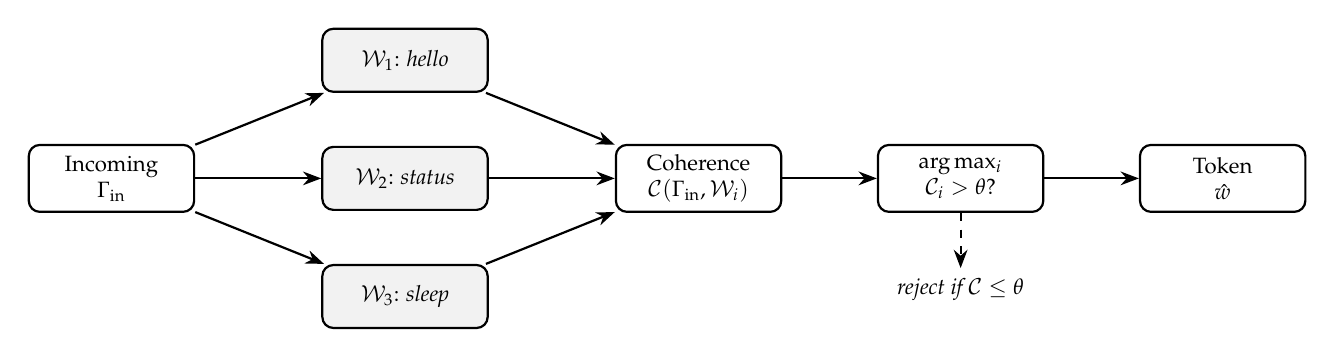
\begin{tikzpicture}[
    node distance=0.7cm and 1.1cm,
    every node/.style={font=\footnotesize},
    box/.style={rectangle, draw, thick, rounded corners, align=center,
                minimum width=2.1cm, minimum height=0.85cm, fill=white},
    basin/.style={rectangle, draw, thick, rounded corners, align=center,
                  minimum width=2.1cm, minimum height=0.8cm, fill=gray!10},
    arr/.style={-{Stealth}, thick},
    darr/.style={-{Stealth}, thick, dashed}
]
\node[box]   (gamma) {Incoming\\$\Gamma_{\mathrm{in}}$};

\node[basin, right=1.6cm of gamma, yshift=1.5cm]  (w1) {$\mathcal{W}_1$: \textit{hello}};
\node[basin, right=1.6cm of gamma]                  (w2) {$\mathcal{W}_2$: \textit{status}};
\node[basin, right=1.6cm of gamma, yshift=-1.5cm] (w3) {$\mathcal{W}_3$: \textit{sleep}};

\node[box, right=1.6cm of w2] (coh) {Coherence\\$\mathcal{C}(\Gamma_{\mathrm{in}},\mathcal{W}_i)$};
\node[box, right=1.2cm of coh] (argmax) {$\arg\max_i$\\$\mathcal{C}_i > \theta$?};
\node[box, right=1.2cm of argmax] (out) {Token\\$\hat{w}$};

\draw[arr] (gamma) -- (w1);
\draw[arr] (gamma) -- (w2);
\draw[arr] (gamma) -- (w3);
\draw[arr] (w1) -- (coh);
\draw[arr] (w2) -- (coh);
\draw[arr] (w3) -- (coh);
\draw[arr] (coh) -- (argmax);
\draw[arr] (argmax) -- (out);
\draw[-{Stealth}, thick, dashed] (argmax.south) -- ++(0,-0.7) node[below, font=\footnotesize\itshape]{reject if $\mathcal{C} \leq \theta$};
\end{tikzpicture}
\caption{Trajectory resonance recognition. The incoming trajectory $\Gamma_{\mathrm{in}}$ is compared against all stored word basins by the DTW coherence functional \eqref{eq:dtw}. Recognition collapses onto the basin with maximal coherence exceeding threshold $\theta$; trajectories with no basin above threshold are rejected. No classifier, no softmax: recognition is geometric collapse.}
\label{fig:recognition}
\end{figure}

\subsection{Trajectory Equivalence Across Modalities}

The trajectory formulation extends the prosodic equivalence of Section~5 into the temporal domain. A sequence of Hyperbionic text tokens $\{T_i\}$ with parameter vectors $\{p_i\}$ defines a discrete path in typographic parameter space:

\begin{equation}
\Gamma_{\mathrm{text}} = \{p_i\}_{i=1}^N.
\label{eq:Gtext}
\end{equation}

The equivalence \eqref{eq:equiv} then extends to trajectories:

\begin{equation}
\Gamma_{\mathrm{audio}} \;\sim\; \Gamma_{\mathrm{mem}} \;\sim\; \Gamma_{\mathrm{text}},
\label{eq:trajequiv}
\end{equation}

where equivalence is defined by preservation of prosodic invariants under projection. Speech-to-text is the operation $\Gamma_{\mathrm{audio}} \to \Gamma_{\mathrm{text}}$; text-to-speech is its inverse. Both are instances of trajectory reconstruction across modalities.


\section{From Salience Packets to Modal Trajectories}

The measurement operator $\mathcal{M}$, as previously defined, presents prosody as a direct mapping from waveform to vector. In practice, this mapping factors through a more primitive layer: a stream of discrete acoustic events. These events form the true substrate of the system, from which both statistical summaries and trajectories are derived. Formalizing this intermediate layer clarifies why the vector is not the fundamental object of the system, and motivates the trajectory representation as a natural consequence of event-based sampling rather than an additional design choice.

\subsection{The Salience Packet as Fundamental Unit}

The Marine processor does not sample the waveform uniformly. It samples \emph{events}: local maxima of the signal that exceed the clip threshold and satisfy the period validity gate. Each detected peak emits a \emph{salience packet}

\begin{equation}
\mathcal{P}_k = \bigl(j_p(k),\; j_a(k),\; h(k),\; s(k),\; E(k),\; t_k\bigr),
\label{eq:packet}
\end{equation}

where $j_p(k)$ is period jitter, $j_a(k)$ is amplitude jitter, $h(k)$ is harmonic alignment, $s(k)$ is the salience score, $E(k) = a_k^2$ is local peak energy, and $t_k$ is the sample index of the peak. The full output of the processor on a waveform segment is the ordered packet stream

\begin{equation}
u(t) \;\longrightarrow\; \{\mathcal{P}_k\}_{k=1}^N.
\label{eq:stream}
\end{equation}

This event-based representation has three properties that distinguish it from uniform sampling. It is \emph{sparse}: packets are emitted only at peaks, so the stream has $N \ll T \cdot f_s$ elements for a waveform of duration $T$. It is \emph{physically grounded}: every component of $\mathcal{P}_k$ is a measured invariant of the signal, not a learned abstraction. And it is \emph{approximately rate-invariant}: because peaks are detected by local comparison rather than by absolute time index, two recordings of the same utterance at different speaking rates produce packet streams with similar jitter profiles but different lengths, which is exactly the structure that the DTW coherence functional in Section~7 is designed to exploit.

The prosodic vector $\mathcal{M}(u)$ defined in equation~\eqref{eq:Mvec} is now revealed as an \emph{aggregation} of the packet stream rather than a direct measurement:

\begin{equation}
\mathcal{M}(u) = \mathcal{A}\bigl(\{\mathcal{P}_k\}_{k=1}^N\bigr),
\label{eq:agg}
\end{equation}

where $\mathcal{A}$ computes the component-wise statistics (means, standard deviations, density, energy mean) defined in \eqref{eq:Mvec}. The two-stage chain is then

\begin{equation}
u(t)
\;\xrightarrow{\;\text{peak detection}\;}
\{\mathcal{P}_k\}
\;\xrightarrow{\;\mathcal{A}\;}
\mathcal{M}(u)
\;\xrightarrow{\;Q\;}
Z_\alpha \in \mathbb{Z}_{Q8.8}^8,
\label{eq:fullchain}
\end{equation}

making explicit that the packet stream is the primary object and the prosodic vector is a secondary, aggregate summary.

\subsection{Packet-to-Modal Projection}

The aggregation route \eqref{eq:agg} collapses temporal information: a vector $\mathcal{M}(u)$ contains no record of \emph{when} within the utterance each packet was emitted. For identity and emotion classification this may be acceptable, but for trajectory-based speech recognition it is not. The alternative is to project each packet individually into a modal coordinate:

\begin{equation}
Z_\alpha(t_k) = Q\bigl(\phi(\mathcal{P}_k)\bigr) \in \mathbb{Z}_{Q8.8}^8,
\label{eq:perpacket}
\end{equation}

where $\phi : \mathcal{P}_k \mapsto \mathbb{R}^8$ selects and possibly augments the packet components. A natural choice includes the six packet fields plus two local-variation terms:

\begin{equation}
\phi(\mathcal{P}_k) = \bigl(j_p(k),\; j_a(k),\; h(k),\; s(k),\; \rho(k),\; E(k),\; \Delta j_p(k),\; \Delta j_a(k)\bigr),
\label{eq:phi}
\end{equation}

where $\rho(k)$ is the instantaneous peak density estimated in a short window around $t_k$, and $\Delta j_p(k) = j_p(k) - j_p(k-1)$, $\Delta j_a(k) = j_a(k) - j_a(k-1)$ are first differences capturing local acceleration of jitter. The per-packet projection \eqref{eq:perpacket} produces a sequence of modal vectors indexed by peak time, from which the trajectory $\Gamma = \{Z_\alpha(t_k)\}_{k=1}^N$ is directly obtained. The three-level hierarchy is then

\begin{align}
\text{Local (event physics):} \quad &\mathcal{P}_k, \notag\\
\text{Global (statistical identity):} \quad &\mathcal{M}(u) = \mathcal{A}(\{\mathcal{P}_k\}), \label{eq:hierarchy}\\
\text{Temporal (trajectory meaning):} \quad &\Gamma = \{Z_\alpha(t_k)\}_{k=1}^N. \notag
\end{align}

All three representations derive from the same packet stream. They are not competing descriptions but projections of the packet stream onto different summary statistics.

\subsection{The SalienceMarker Enumeration as Topological Signal}

The Marine processor does not emit only packets. Its output type is the enumeration

\begin{equation}
\mathrm{SalienceMarker} \in \{\mathrm{Peak}(\mathcal{P}_k),\; \mathrm{Fracture},\; \mathrm{Noise},\; \mathrm{Insufficient}\},
\label{eq:marker}
\end{equation}

where $\mathrm{Fracture}$ marks silence or a gap in the signal (inter-peak period exceeding the validity gate), $\mathrm{Noise}$ marks a region of high-amplitude aperiodic signal (energy above the clip threshold but no coherent peaks), and $\mathrm{Insufficient}$ marks a region where the processor has not yet warmed up. This enumeration introduces topological structure into the signal: rather than a continuous function, the processor produces a partition of the timeline into structured regions (voiced, voiced-unstable), boundaries (fractures between voiced regions), and noise fields.

The Fracture marker is particularly important for the trajectory architecture. A trajectory $\Gamma$ is a sequence of modal coordinates at peak times; a Fracture between two peaks creates a gap in the sequence that is not filled by interpolation. Word basins $\mathcal{W}_i$ therefore naturally encode the silence structure of the corresponding utterance, and the DTW alignment path $\pi$ in equation~\eqref{eq:dtw} must skip over Fracture gaps in both the query and the stored basin consistently. The Fracture marker therefore induces a canonical decomposition of any trajectory into voiced components separated by silence boundaries:
\begin{equation}
\Gamma = \bigsqcup_{m} \Gamma_m,
\label{eq:decomp}
\end{equation}
where each $\Gamma_m$ is a connected voiced segment and $\sqcup$ denotes disjoint union. DTW alignment is restricted to pairs within the same component; TARTAN tiles inherit this segmentation, with boundary flags $b_{\ell,j}$ propagating the Fracture structure up the hierarchy. In the Hyperbionic rendering, Fracture events correspond to typographic white space: the absence of prosodic transformation between adjacent tokens is itself a prosodic signal. The system thus maintains a clean distinction between two kinds of absence: silence removes points from $\Gamma$ entirely (a topological gap in the trajectory), while low salience down-weights existing points in $\mathcal{C}$ without removing them (a geometric thinning of the trajectory). Conflating these two would misclassify quiet expressive passages as silence; the Fracture marker prevents this by requiring energy to fall below the clip threshold, not merely for salience to be low.

\section{A Real Trajectory Space and TARTAN Multiscale Tiling}

\noindent\textit{This section establishes the real geometric structure of trajectory space and introduces a multiscale organization required for stability. Raw trajectories are sensitive to local perturbations; TARTAN constructs a hierarchy that preserves global structure while isolating local noise, allowing recognition to operate at the appropriate scale. Its role is not compression but stabilization.}


The trajectory representation $\Gamma = \{Z_\alpha(t_k)\}$ is powerful but fragile in a specific way: a small perturbation in a single packet---a spurious peak, a momentary noise spike---can shift the trajectory locally and degrade DTW coherence. A robust architecture requires a multiscale organization that separates global word shape from local packet noise.

\subsection{The Real Trajectory Space}

Before introducing the multiscale structure, it is useful to state the trajectory space precisely. After rescaling the fixed-point vectors to real values, each modal coordinate is an element of $V = \mathbb{R}^8$, and the inner product is the ordinary real dot product

\begin{equation}
\langle Z, Z' \rangle = \sum_{i=1}^{8} Z_i Z'_i.
\label{eq:ip}
\end{equation}

No imaginary components are required.

\begin{proposition}[Geometric Phase Representation]
Let $\Gamma \subset \mathbb{R}^8$ be a trajectory in modal space $V$. All phase-dependent interference effects are representable as geometric relations on $\Gamma$ under the real inner product structure of $V$. No complex extension is required.
\end{proposition}

Phase mismatch corresponds to trajectory divergence under alignment: two trajectories that would destructively interfere in a complex-exponential model appear as misaligned paths under the DTW coherence functional, yielding low or negative $\mathcal{C}$. Phase-like structure is represented geometrically by the direction of trajectory movement through modal space, not by imaginary coefficients. The space of finite trajectories of any length is $\mathcal{T} = \bigcup_{N \geq 1} V^N$, and the normalized coherence between two trajectories under an alignment path $\pi$ is

\begin{equation}
\mathcal{C}(\Gamma, \Gamma') = \frac{1}{|\pi|} \sum_{(k,\ell) \in \pi} \frac{\langle Z_\alpha(t_k), Z'_\alpha(t_\ell) \rangle}{\|Z_\alpha(t_k)\| \cdot \|Z'_\alpha(t_\ell)\| + \varepsilon},
\label{eq:Cnorm}
\end{equation}

where $\varepsilon > 0$ prevents division by zero for silent or near-zero packets. The coherence is in $[-1, 1]$, with $\mathcal{C} = 1$ indicating perfect alignment and $\mathcal{C} \leq 0$ indicating destructive interference: the two trajectories are moving in incompatible directions in modal space at the aligned time steps.

\subsection{TARTAN: Trajectory-Aware Recursive Tiling with Annotated Noise}

A raw trajectory $\Gamma = \{Z_\alpha(t_k)\}_{k=1}^N$ operates at the finest temporal scale---one modal vector per detected peak. For recognition, retrieval, and storage, it is advantageous to organize this fine-grained sequence into a hierarchy of coarser approximations. The TARTAN framework provides this organization.

TARTAN maps a raw trajectory to a sequence of tiled approximations at increasing coarseness levels:

\begin{equation}
\Gamma \;\longrightarrow\; \mathcal{T}_0(\Gamma),\; \mathcal{T}_1(\Gamma),\; \ldots,\; \mathcal{T}_L(\Gamma),
\label{eq:tartan}
\end{equation}

where $\mathcal{T}_0(\Gamma) = \Gamma$ is the original packet-level trajectory and each $\mathcal{T}_{\ell+1}$ is obtained by recursively tiling $\mathcal{T}_\ell$: partitioning it into non-overlapping segments and replacing each segment with a local summary tile

\begin{equation}
\tau_{\ell,j} = \bigl(\bar{Z}_{\ell,j},\; \Sigma_{\ell,j},\; \eta_{\ell,j},\; b_{\ell,j}\bigr),
\label{eq:tile}
\end{equation}

where $\bar{Z}_{\ell,j}$ is the mean modal vector over the segment, $\Sigma_{\ell,j}$ is a scalar or diagonal measure of local variance, $\eta_{\ell,j}$ is an annotated noise estimate (derived from the Noise markers in the SalienceMarker stream), and $b_{\ell,j} \in \{0, 1\}$ is a boundary flag marking whether a Fracture occurred within the segment.

The boundary flag is the key innovation: by propagating Fracture information up the tiling hierarchy, TARTAN ensures that silence structure is preserved at every scale. A coarse tile spanning a silence boundary is annotated as such, so that alignment at the coarse level does not inadvertently match voiced content across a silence gap.

Multiscale recognition proceeds by computing a weighted coherence across levels:

\begin{equation}
\mathcal{C}_{\mathrm{TARTAN}}(\Gamma, \Gamma') = \sum_{\ell=0}^{L} w_\ell\, \mathcal{C}\bigl(\mathcal{T}_\ell(\Gamma),\; \mathcal{T}_\ell(\Gamma')\bigr),
\label{eq:Ctartan}
\end{equation}

where the weights satisfy
\begin{equation}
\sum_{\ell=0}^{L} w_\ell = 1, \qquad w_0 \geq w_1 \geq \cdots \geq w_L > 0,
\label{eq:tartanweights}
\end{equation}
enforcing coarse-to-fine dominance. This normalization ensures that $\mathcal{C}_{\mathrm{TARTAN}} \in [-1, 1]$ whenever each level coherence is normalized, and the monotone decrease prevents fine-level packet noise from destabilizing recognition. At coarse levels the system detects global word shape; at fine levels it verifies local prosodic microstructure. Recognition requires $\mathcal{C}_{\mathrm{TARTAN}}(\Gamma, \mathcal{W}_i) > \theta$ for a stored word basin $\mathcal{W}_i$.

\subsection{The Complete Equivalence}

With all components in place, the full processing pipeline is

\begin{equation}
u(t)
\;\xrightarrow{\;\text{Marine}\;}
\{\mathcal{P}_k\}
\;\xrightarrow{\;\phi, Q\;}
\{Z_\alpha(t_k)\}
\;\xrightarrow{\;\text{TARTAN}\;}
\{\mathcal{T}_\ell(\Gamma)\}_{\ell=0}^{L},
\label{eq:pipeline}
\end{equation}

and the Hyperbionic visual trajectory $\Gamma_{\mathrm{text}} = \{p_i\}$ is a rendering of the same packet-derived structure into typographic parameter space. The equivalence \eqref{eq:trajequiv} therefore extends to include the TARTAN representation:

\begin{equation}
\Gamma_{\mathrm{audio}} \;\sim\; \Gamma_{\mathrm{mem}} \;\sim\; \Gamma_{\mathrm{tartan}} \;\sim\; \Gamma_{\mathrm{text}},
\label{eq:fullequiv}
\end{equation}

where equivalence is preservation of prosodic invariants under admissible projection at each stage. The four components of the system have distinct roles that are now precisely delineated: Marine performs event extraction, MEM$|$8 provides modal storage of quantized packet coordinates, TARTAN organizes trajectories into multiscale tiles that are robust to local packet noise, and Hyperbionic Reading renders the same trajectory structure as a visual field. None of these roles overlaps; each is a necessary stage in the pipeline from acoustic signal to visual prosody.

\begin{figure}[p]
\centering
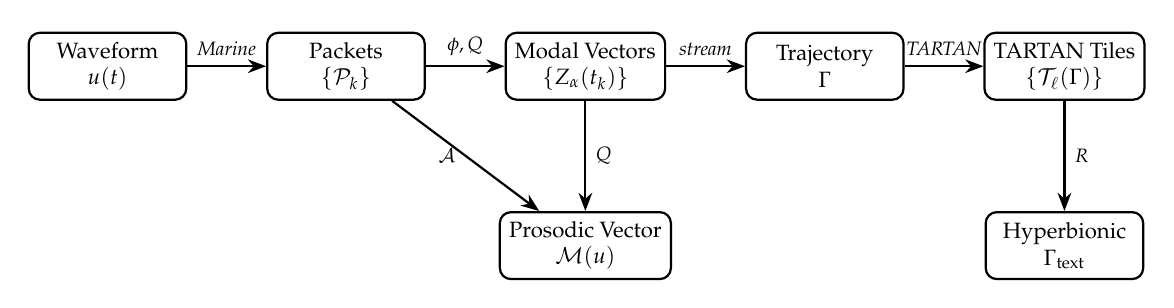
\begin{tikzpicture}[
    node distance=0.7cm and 1.0cm,
    every node/.style={font=\footnotesize},
    box/.style={rectangle, draw, thick, rounded corners, align=center,
                minimum width=2.0cm, minimum height=0.85cm, fill=white},
    arr/.style={-{Stealth}, thick},
    label/.style={font=\scriptsize\itshape, midway, above}
]
\node[box] (audio)   {Waveform\\$u(t)$};
\node[box, right=of audio]  (pkts)  {Packets\\$\{\mathcal{P}_k\}$};
\node[box, right=of pkts]   (modal) {Modal Vectors\\$\{Z_\alpha(t_k)\}$};
\node[box, right=of modal]  (traj)  {Trajectory\\$\Gamma$};
\node[box, right=of traj]   (tartan){TARTAN Tiles\\$\{\mathcal{T}_\ell(\Gamma)\}$};

\node[box, below=1.4cm of modal] (mvec) {Prosodic Vector\\$\mathcal{M}(u)$};
\node[box, below=1.4cm of tartan] (hyper) {Hyperbionic\\$\Gamma_{\mathrm{text}}$};

\draw[arr] (audio)  -- node[label]{Marine} (pkts);
\draw[arr] (pkts)   -- node[label]{$\phi,Q$} (modal);
\draw[arr] (modal)  -- node[label]{stream} (traj);
\draw[arr] (traj)   -- node[label]{TARTAN} (tartan);

\draw[arr] (pkts)   -- node[font=\scriptsize\itshape, left]{$\mathcal{A}$} (mvec);
\draw[arr] (modal)  -- node[font=\scriptsize\itshape, right]{$Q$} (mvec);
\draw[arr] (tartan) -- node[font=\scriptsize\itshape, right]{$R$} (hyper);
\end{tikzpicture}
\caption{Full processing pipeline. The waveform $u(t)$ is converted by the Marine processor into a sparse packet stream $\{\mathcal{P}_k\}$. Per-packet projection $\phi$ followed by quantization $Q$ yields modal vectors; their sequence is the trajectory $\Gamma$. TARTAN organizes $\Gamma$ into a multiscale tile hierarchy. Aggregation $\mathcal{A}$ collapses the packet stream to the prosodic vector $\mathcal{M}(u)$ (statistical identity path). The Hyperbionic rendering operator $R$ projects the tiled trajectory into the visual field.}
\label{fig:pipeline}
\end{figure}


\section{Reconstruction and Cue-Based Retrieval}

The bidirectionality of the framework raises a question about information recovery. Given a Hyperbionic rendering $R(g, p)$, can the original prosodic structure be recovered? The answer depends on which components of $p$ are preserved under rendering and which are collapsed in the visual output.

For the core parameters in Table~\ref{tab:mapping}, the mapping is injective in principle: given a rendered glyph and knowledge of the rendering operator $R$, the parameter vector $p$ can be extracted by inverting the visual-to-parameter correspondences. In practice, quantization and rendering resolution introduce information loss, but the loss is bounded by the same constraints that govern the admissibility of $R$: a rendering that is legible is one that preserves enough visual variation to make the parameter vector recoverable.

This recovery structure corresponds to what Tulving identified as \emph{synergistic ecphory}: the process by which a partial retrieval cue, combined with stored engram information, produces a recollective state that neither the cue nor the engram alone determines~\cite{Tulving1982}. Hyperbionic text functions as a structured cue set for prosodic reconstruction. The rendered glyph is the cue; the stored prosodic vector (or, in the MEM$|$8 case, the modal lattice coordinate) is the engram; and the reconstructed acoustic impression is their joint product. The full reconstruction chain is

\begin{equation}
R(g, p) \;\xrightarrow{\;R^{-1}\;}\; p \;\xrightarrow{\;Q^{-1}\;}\; \mathcal{M}(u) \;\xrightarrow{\;\text{synthesis}\;}\; \hat{u}(t),
\label{eq:recon}
\end{equation}

where $\hat{u}(t)$ is a reconstructed waveform consistent with the recovered prosodic vector. This is not lossless reconstruction of the original waveform---the measurement operator $\mathcal{M}$ is many-to-one, and distinct waveforms with the same prosodic vector are indistinguishable at the level of \eqref{eq:Mvec}---but it is reconstruction of prosodic structure, which is precisely the structure that plain text discards and Hyperbionic rendering preserves.

\section{Constraints and Stability}

The expressive power of the Hyperbionic system must be bounded to remain usable. Without constraints, the parameter space $\mathbb{R}^m$ allows mappings that render text unreadable---glyphs too small to resolve, rotations that invert letterforms, displacements that destroy word boundaries.

Before developing the formal constraints, it is useful to note that the admissibility problem has a precise analogue in the audio domain. Standard lossy codecs (MP3, AAC) apply a psychoacoustic masking model: when a loud transient such as a snare hit occurs immediately before a quiet signal such as a vocal breath, the algorithm discards the quiet signal on the grounds that the loud event masks it. This produces what audio engineers call \emph{spectral fracturing}: metallic ringing, temporal smearing, and pre-echo artifacts that the auditory system registers subconsciously even when the conscious mind cannot identify them. The computational load of repairing the fractured signal blunts emotional impact.

Spectral fracturing is, in the framework of this paper, a pathological aggregation: a codec that discards masked signal components is a system that factors through a lossy version of $\mathcal{A}$, and by the Aggregation Impossibility Proposition the resulting representation cannot recover expressive coherence $\chi$. What is destroyed is precisely the structured microdynamic jitter that carries the emotional carrier wave---the subtle harmonic weight and temporal micro-variation of a human performance that cannot be reconstructed from amplitude and spectral envelope alone. Hyperbionic rendering must avoid the typographic analogue of spectral fracturing: transformations that preserve nominal glyph structure while destroying the coherence required for perceptual integration. An admissible rendering is one that neither collapses prosodic distinctions nor introduces visual artifacts that impose a reconstruction burden on the reader analogous to the cognitive load of a fractured audio signal. The admissibility constraints introduced informally in Section~4 can be stated precisely.

Define the \emph{perceptual validity region} as the set of parameter vectors $p_i$ such that the rendered glyph $R(g_i, p_i)$ is legible at normal reading distance and reading speed. This region is bounded: there exist maximum and minimum values for each parameter beyond which legibility fails. Within this region, the constraint energy

\begin{equation}
C[p] = \int_{\mathcal{M}} \left(\alpha\, \theta(x)^2 + \beta\, S(x)^2 + \gamma\, \xi(x)^2\right) d\mu(x)
\label{eq:Cp}
\end{equation}

---where $\theta$ measures misalignment between the rendering trajectory and the salience gradient, $S$ measures uncertainty in parameter values, and $\xi$ measures rotational instability in the visual field---is bounded above by a legibility threshold $C_{\max}$. Admissible renderings satisfy $C[p] \leq C_{\max}$.

The legibility constraint has a further consequence: it implies that Hyperbionic rendering operates on a low-dimensional admissible manifold within the full parameter space. Not all combinations of the parameters in \eqref{eq:pi} are jointly admissible; the constraints couple the parameters and restrict the system to a structured subset of $\mathbb{R}^m$. This is the typographic analogue of the biological prior in cognitive trajectory models: the system does not search the full parameter space uniformly but is confined by legibility and stability constraints to a lower-dimensional structured region.

The perceptual weights $w_i$ in the $G$-metric are not universal but listener-variable. A relevant empirical observation is that audiometric studies have reported that women, on average, exhibit approximately 2 dB greater sensitivity than men across frequency ranges, a difference attributed to evolutionary pressures related to detecting the high-frequency cues of infant distress. If this differential sensitivity is real and of the reported magnitude, it has a direct consequence for spectral fracturing: compression artifacts that fall below the conscious detection threshold of a less sensitive auditory system may register supra-threshold for a more sensitive one, imposing a subconscious cognitive load on the listener that blunts emotional impact. In the framework of this paper, this corresponds to listener-specific $G$-metrics with higher weights on the dimensions most affected by compression artifacts---temporal fine structure and high-frequency harmonic content. A Hyperbionic rendering system that aims to preserve emotional impact across a diverse listener population must therefore parameterize $G$ as a function of the target perceptual profile, not treat it as a fixed universal constant. The claim about 2 dB differential sensitivity is taken from existing discourse on this topic and should be understood as an empirical hypothesis requiring controlled audiometric validation rather than an established universal constant; the structural point about listener-variable $G$-metrics holds independently of the specific magnitude. The system must therefore treat $G$ as a parameterized perceptual model rather than a fixed metric, adapting the weighting structure to the sensitivity profile of the target observer.


\section{Implementation: The Marine Processor as $\mathcal{M}$ in Practice}

The measurement operator $\mathcal{M}$ defined in Section~2 is not merely a formal object. It has a concrete, running implementation in the Marine processor, a Rust library designed for $O(1)$ per-sample operation. Examining the implementation reveals three places where the formal definition and the executable code diverge in instructive ways, and one where the implementation makes a stronger architectural commitment than the formalism requires.

\subsection{Exponential Moving Average versus Window Mean}

The formal definition of period jitter uses sample means: $j_p(k) = |\Delta t_k - \overline{\Delta t}| / \overline{\Delta t}$, where $\overline{\Delta t}$ is the mean inter-peak interval over all observed peaks. This is clean mathematically but impractical for real-time processing, since computing the sample mean requires storing all past periods and updating a running sum---operations that are $O(N)$ in memory if not time.

The implementation replaces the sample mean with an exponential moving average (EMA). Let $\mu_k$ denote the EMA of inter-peak periods after the $k$-th peak. The update rule is

\begin{equation}
\mu_k = \alpha_p \cdot \Delta t_k + (1 - \alpha_p) \cdot \mu_{k-1},
\label{eq:ema}
\end{equation}

where $\alpha_p \in (0,1)$ is the EMA smoothing coefficient configured at initialization. Jitter is then computed as $j_p(k) = |\Delta t_k - \mu_{k-1}| / \mu_{k-1}$, using the previous EMA value as the reference rather than the global mean. An identical EMA $\mu^a_k$ tracks peak amplitudes for the amplitude jitter computation.

The classical definition of jitter assumes a stationary reference distribution. This assumption is violated in natural speech, where fundamental frequency drifts continuously over time. The EMA formulation replaces a global reference with a locally adaptive one, allowing the system to track prosodic intent rather than penalize it as deviation. The substitution is therefore not an optimization but a correction to the measurement model itself: the formal definition in equation~\eqref{eq:Mvec} should be read as using a weighted mean with exponential decay rather than a uniform sample mean. A speaker who gradually lowers their pitch will show low EMA-based jitter throughout, correctly identifying the signal as locally periodic despite global drift; the sample-mean version would misclassify the drift as instability.

The EMA also implements the warmup condition implicitly. The processor exposes an \texttt{is\_warmed\_up()} predicate that returns true only when at least three peaks have been detected and the EMA has received enough updates to be reliable. Formally, this means that $\mathcal{M}(u)$ is a partial function: it is undefined on waveforms too short to contain at least three peaks satisfying the minimum period constraint. The sliding window $\gamma(t) = \mathcal{M}(u\!\upharpoonright_{[t-\Delta, t]})$ introduced in Section~7 therefore requires a window width $\Delta$ satisfying

\begin{equation}
\Delta \geq \frac{3}{f_0},
\label{eq:warmup}
\end{equation}

where $f_0$ is the fundamental frequency of the signal. For speech at 100--300 Hz, this constrains $\Delta \geq 10$--$30$ milliseconds---a natural lower bound that the implementation enforces implicitly through the warmup predicate.

\subsection{The Harmonic Coherence Placeholder}

The formal vector \eqref{eq:Mvec} includes a harmonic coherence component $h$ measuring the degree of periodic regularity in the voiced signal. In the current implementation, this component is hardcoded to $h = 1.0$ with a comment marking it as a TODO item: \enquote{Harmonic score (simplified -- TODO: FFT-based detection). For now, assume voiced content.}

This means the implementation currently computes a seven-dimensional effective vector, not an eight-dimensional one. The eighth dimension---harmonic coherence---is present structurally but carries no information. The salience score $s = 1/(1 + j_p + j_a)$ is consequently computed from jitter alone, without any contribution from spectral periodicity. Signals with strong harmonic structure (sustained vowels) and signals with weak harmonic structure (fricatives, noise) receive the same $h$ value and are distinguished only by their jitter profiles.

The intended extension is FFT-based harmonic detection: computing the ratio of energy at the fundamental frequency and its harmonics to total signal energy, which gives a value in $[0,1]$ that approaches 1 for purely periodic signals and 0 for white noise. Formally,

\begin{equation}
h = \frac{\sum_{k=1}^{K} |U(k f_0)|^2}{\int_0^{f_s/2} |U(f)|^2\, df},
\label{eq:h}
\end{equation}

where $U(f)$ is the discrete Fourier transform of a windowed segment of $u(t)$, $f_0$ is the estimated fundamental frequency, and $K$ is the number of harmonics included. This computation is $O(N \log N)$ per window rather than $O(1)$ per sample, which is why it has not yet been integrated: it would require a hybrid architecture in which the peak-based $O(1)$ processor feeds a periodic FFT-based harmonic estimator operating on a longer lookback buffer.

The formal framework anticipates this extension naturally. The measurement operator $\mathcal{M}$ is defined abstractly as a map to $\mathbb{R}^n$; the specific components are a concrete instance, not a structural constraint. Adding a genuinely computed $h$ component does not change the architecture of the Hyperbionic system---the equivalence \eqref{eq:equiv} holds for any prosodic parameter vector, regardless of dimensionality---but it does change the information content of the modal coordinate $Z_\alpha$ and therefore the discriminative power of the trajectory resonance recognizer. Utterances that are currently indistinguishable (same jitter profiles, different harmonic structure) would become distinguishable once $h$ is measured rather than assumed. Until this component is implemented, the system operates in a reduced discriminative regime in which periodicity is inferred indirectly through jitter rather than measured explicitly. This is a structural limitation of the current implementation, not merely an engineering detail.

\section{Operational Constraints and Real-Time Geometry}

The Marine processor enforces two further constraints that have formal analogues in the measurement operator's domain of definition: a period validity gate and a clip threshold.

\subsection{Period Validity Gate}

The processor accepts a peak contribution only when the inter-peak period falls within a configurable range $[\texttt{min\_period}, \texttt{max\_period}]$ specified in samples. This gate serves two purposes: it excludes spurious detections (very short periods corresponding to noise spikes) and it excludes silence gaps (very long periods corresponding to pauses between utterances). Formally, let $f_s$ denote the sample rate. The gate defines an admissible frequency range

\begin{equation}
f_{\min} = \frac{f_s}{\texttt{max\_period}}, \qquad f_{\max} = \frac{f_s}{\texttt{min\_period}},
\label{eq:frange}
\end{equation}

and the measurement operator is defined only on signal segments whose instantaneous fundamental frequency lies within $[f_{\min}, f_{\max}]$. For the default speech configuration at 22050 Hz, typical values confine the operator to voiced fundamental frequencies in the speech range, rejecting both subsonic artifacts and aliased high-frequency noise.

The period gate has a geometric interpretation in trajectory space. A trajectory $\Gamma = \{Z_\alpha(t_k)\}$ is defined only at time steps where a valid peak is detected within the admissible period range. At time steps where the signal is silent, unvoiced, or outside the frequency range, the trajectory is undefined---the point is simply absent from the sequence. This means that word basins $\mathcal{W}_i$ are sparse trajectories: sequences of modal coordinates at the times of valid peaks, with gaps corresponding to unvoiced or silent intervals. The DTW coherence functional \eqref{eq:dtw} must be understood as aligning sparse sequences, not dense time series, which the standard DTW algorithm handles naturally through its admissible alignment path constraint.

\subsection{Clip Threshold as a Pre-Gate}

Before any peak detection is attempted, the processor applies a clip threshold: samples with absolute value below \texttt{clip\_threshold} are ignored entirely, bypassing even the peak detection logic. This is a pre-gate that defines the silence floor of the system.

Formally, let $\varepsilon_{\mathrm{clip}} > 0$ denote the clip threshold. The effective input to $\mathcal{M}$ is not $u(t)$ itself but the gated signal

\begin{equation}
u_\varepsilon(t) = \begin{cases} u(t) & \text{if } |u(t)| \geq \varepsilon_{\mathrm{clip}}, \\ 0 & \text{otherwise.} \end{cases}
\label{eq:gate}
\end{equation}

The measurement operator $\mathcal{M}$ acts on $u_\varepsilon$, not on $u$. This means that very quiet passages---below the noise floor of the recording environment---contribute no peaks and no trajectory points. The clip threshold is therefore the operational definition of silence in the Marine framework: a continuous segment on which $u(t)$ lies entirely below $\varepsilon_{\mathrm{clip}}$ produces no output from $\mathcal{M}$, and its absence from the trajectory is the signal that a silence or unvoiced interval has occurred.

In the Hyperbionic context, this gating has a direct typographic correlate. Tokens in a transcript that correspond to silent intervals---pauses, breaths, hesitations---receive no prosodic parameter vector from $\mathcal{M}$, and so their Hyperbionic rendering falls back to the default glyph $R(g_i, \mathbf{0})$: unstyled, unmodified text. Silence becomes the absence of typographic transformation, which is the correct rendering: a pause in speech is marked in Hyperbionic text by the surrounding white space, not by any active visual property of the adjacent glyphs.


\section{Beyond the Audible-Stable Regime: Haptic Extension and Expressive Deviation}

\noindent\textit{This section removes two simplifying assumptions of the preceding framework: that all relevant structure lies within the audible band, and that deviation from periodicity is noise. Both assumptions exclude meaningful signal. The extensions introduced here incorporate sub-audible somatic structure and reinterpret deviation as a carrier of intention, completing the invariant field.}


The formulation developed thus far assumes that prosodic structure is captured by stable periodic features within the audible frequency band. This assumption is both physically and perceptually incomplete in two orthogonal directions. First, acoustic signals below approximately 40 Hz are not primarily perceived auditorily but somatically, as vibration felt in the chest, body, and surrounding environment. Second, the salience formula $s = 1/(1 + \overline{j_p} + \overline{j_a})$ treats all jitter as degradation, which is correct for detecting synthetic or damaged signals but wrong for expressive performance, where controlled deviation is the carrier of meaning. What was previously classed as noise occupies exactly the dimensions where intention lives.

\subsection{Infrasound and the Haptic Channel}

The Marine configuration gates the measurement operator to an admissible frequency range $[f_{\min}, f_{\max}]$ corresponding to roughly 60--4000 Hz for speech. Signals below $\sim 40$ Hz are discarded. But low-frequency content below the auditory threshold is not absent from musical and environmental signals: the sub-bass of a bass guitar, the chest-felt pulse of a kick drum, the room pressure of a large acoustic space are all real physical quantities that carry structural information about the source and environment.

Let $u(t)$ be decomposed spectrally into
\begin{equation}
u(t) = u_{\mathrm{aud}}(t) + u_{\mathrm{infra}}(t),
\label{eq:decomp_freq}
\end{equation}
where $u_{\mathrm{infra}}$ contains components with instantaneous frequency $f < 40$ Hz. The current measurement operator $\mathcal{M}$ acts only on $u_{\mathrm{aud}}$. We define the extended measurement operator
\begin{equation}
\widetilde{\mathcal{M}}(u) = \bigl(\mathcal{M}(u_{\mathrm{aud}}),\; H(u_{\mathrm{infra}})\bigr),
\label{eq:Mtilde}
\end{equation}
where $H$ is a \emph{haptic measurement functional} extracting the low-frequency envelope:
\begin{equation}
H(u_{\mathrm{infra}}) = \bigl(A_{\mathrm{lf}},\; \sigma_{\mathrm{lf}},\; \nabla A_{\mathrm{lf}}\bigr).
\label{eq:H}
\end{equation}
Here $A_{\mathrm{lf}}$ is the low-frequency energy envelope, $\sigma_{\mathrm{lf}}$ its temporal variance, and $\nabla A_{\mathrm{lf}}$ its rate of change. These quantities encode perceived pressure, pulsation rate, and environmental resonance---the somatic correlates of musical bass.

The haptic channel is structurally distinct from the auditory channel in two respects. Perceptually, infrasound is field-like: it is felt across the whole body rather than localized in the auditory system, and the relevant spatial scale is the body or room rather than the cochlea. This means that in the Hyperbionic rendering, infrasound does not map to glyph-level deformation but to \emph{global layout modulation}---baseline drift, field-wide spacing variation, or background texture---reflecting the distributed rather than localized nature of somatic perception. Formally, the trajectory space extends to $V = \mathbb{R}^{8+3}$, with the three haptic dimensions decoupled from the $G$-metric of the auditory dimensions and requiring separate perceptual weighting.

\subsection{Structured Jitter as Expressive Signal}

Jitter, in the current framework, is defined as deviation from an exponentially weighted expected period. But this definition conflates two categorically different phenomena. Random jitter arises from measurement noise, imprecise articulation, or signal degradation: it has no temporal structure and carries no information beyond the degradation level. Structured jitter arises from intentional expressive modulation: vibrato in a sustained note is periodic jitter; groove in a rhythm section is timing jitter locked to a metrical grid; the roughness of a distorted guitar is amplitude jitter with a specific spectral signature. These are not corruptions of a periodic signal but features of it.

We decompose the observed jitter sequence $\{j(k)\}$ into two components:
\begin{equation}
j(k) = j_{\mathrm{rand}}(k) + j_{\mathrm{expr}}(k),
\label{eq:jdecomp}
\end{equation}
where $j_{\mathrm{rand}}$ is stochastic and carries no predictive structure, and $j_{\mathrm{expr}}$ is structured, reproducible, and carries expressive information.

\begin{definition}[Expressive Coherence]
Let $\{j(k)\}_{k=1}^N$ be a sequence of jitter measurements and $\{\hat{j}(k)\}$ a locally predicted sequence obtained by fitting a short-memory model to recent values. The \emph{expressive coherence} is
\begin{equation}
\chi = 1 - \frac{\mathrm{Var}\bigl(j(k) - \hat{j}(k)\bigr)}{\mathrm{Var}\bigl(j(k)\bigr)},
\label{eq:chi}
\end{equation}
with $\chi \in [0, 1]$: $\chi \approx 1$ when deviation follows a predictable pattern, $\chi \approx 0$ when deviation is indistinguishable from white noise.
\end{definition}

High $\chi$ at substantial $\overline{j}$ indicates expressive performance. Low $\chi$ at substantial $\overline{j}$ indicates damage or noise. Low $\chi$ at low $\overline{j}$ indicates a synthetic or mechanically regular signal. The original scalar salience $s$ cannot distinguish the first from the third of these cases when mean jitter happens to be comparable; the expressive coherence $\chi$ distinguishes all three.

We define a second salience axis
\begin{equation}
s_{\mathrm{expr}} = \chi \cdot (\overline{j_p} + \overline{j_a}),
\label{eq:sexpr}
\end{equation}
measuring the magnitude of structured deviation: it is large when jitter is both substantial and organized. The full salience representation is then two-dimensional:
\begin{equation}
\mathbf{s} = (s_{\mathrm{stable}},\; s_{\mathrm{expr}}),
\label{eq:s2d}
\end{equation}
where $s_{\mathrm{stable}} = s = 1/(1 + \overline{j_p} + \overline{j_a})$ is the existing periodicity salience and $s_{\mathrm{expr}}$ is the new expressive axis. Stable periodic signals maximize $s_{\mathrm{stable}}$; expressive signals maximize $s_{\mathrm{expr}}$; synthetic or damaged signals minimize both.

The two-dimensional salience space has an important application to the authentication of human performance. A human vocal performance is produced by a coupled physical system: lungs, diaphragm, vocal cords, resonant cavities, and neural motor control all constrain the jitter profile jointly. The resulting jitter is not random but structured by physiology---it lies near the constraint manifold of a biological dynamical system. We call this property \emph{biological coupling}: the jitter sequence is organized by a physical process that imposes internal consistency across time scales from milliseconds (glottal pulse variation) to seconds (respiratory cycle). Generative audio synthesis systems, by contrast, produce jitter by sampling from learned distributions over spectral and temporal features. The resulting jitter is \emph{decoupled}: it may match the marginal statistics of human jitter (mean, variance, spectral envelope) while failing to reproduce the coupled temporal structure. In the framework of this paper, biological coupling corresponds to high $\chi$ with a structured manifold, while decoupled synthetic jitter produces low $\chi$ despite superficially plausible amplitude and pitch.

\begin{proposition}[Biological Coupling Detectability]
Let $u_{\mathrm{human}}$ be a human vocal performance and $u_{\mathrm{synth}}$ a generative synthesis of the same utterance. If the synthesis system matches the aggregate statistics $\mathcal{M}(u_{\mathrm{human}}) \approx \mathcal{M}(u_{\mathrm{synth}})$ but does not model the physiological coupling of the human jitter process, then $\chi(u_{\mathrm{human}}) \gg \chi(u_{\mathrm{synth}})$ and the two signals are distinguishable by trajectory coherence even when indistinguishable by aggregate prosodic statistics.
\end{proposition}

This proposition provides the mathematical basis for biometric voice authentication via expressive coherence: the structured biological jitter of a human performance is not merely a stylistic feature but a physically grounded invariant that aggregate-matching synthesis cannot replicate without modeling the underlying physiology. This establishes a separation principle: synthesis systems that match marginal statistics but fail to reproduce coupled temporal structure remain distinguishable under trajectory-based metrics. A voice authentication system based on $\chi$ is therefore resistant to attacks that match spectral envelope, pitch contour, and mean jitter while lacking the physiological coupling that generates structured temporal coherence in human performance.

\begin{proposition}[Aggregation Information Loss]
The aggregation map $\mathcal{A}$ is not injective on trajectories: $\mathcal{A}(\Gamma_1) = \mathcal{A}(\Gamma_2)$ does not imply $\Gamma_1 = \Gamma_2$. Therefore any system that operates exclusively on $\mathcal{M}(u) = \mathcal{A}(\{\mathcal{P}_k\})$ cannot recover trajectory curvature or expressive coherence $\chi$.
\end{proposition}

\hyperemph{This is not a limitation of any particular model design but a general impossibility result for the class of representations that factor through $\mathcal{A}$.} Standard acoustic embedding systems, which map utterances to fixed-length vectors derived from averaged or pooled features, belong to this class. The trajectory-based architecture proposed here does not factor through $\mathcal{A}$, and so is not subject to this limitation.

\subsection{Reinterpretation of Annotated Noise in TARTAN}

Under the original formulation, the annotated noise field $\eta_{\ell,j}$ in each TARTAN tile records structured deviation to be tracked and, implicitly, suppressed or normalized away. The decomposition \eqref{eq:jdecomp} and the expressive coherence \eqref{eq:chi} permit a more discriminating treatment. Each tile is extended to
\begin{equation}
\tau_{\ell,j} = \bigl(\bar{Z}_{\ell,j},\; \Sigma_{\ell,j},\; \eta_{\ell,j},\; \chi_{\ell,j},\; b_{\ell,j}\bigr),
\label{eq:tileext}
\end{equation}
where $\chi_{\ell,j}$ is the expressive coherence computed over the packets within tile $(\ell, j)$. The noise field $\eta_{\ell,j}$ and coherence $\chi_{\ell,j}$ together classify tile content:
\begin{align}
\eta \approx 0,\; \chi \approx 0 &\;\Rightarrow\; \text{silence or highly stable signal,} \notag\\
\eta > 0,\; \chi \approx 0 &\;\Rightarrow\; \text{noise or damaged signal,} \label{eq:classification}\\
\eta > 0,\; \chi \approx 1 &\;\Rightarrow\; \text{expressive signal.} \notag
\end{align}
This classification replaces the binary noise/signal distinction with a ternary structure that can represent the full range from mechanical precision through expressive performance to genuine noise---three regimes that were previously conflated whenever mean jitter values happened to agree.

\subsection{Example: Robotic versus Expressive Utterance}

To make the extended framework concrete, consider two realizations of the same lexical item that are indistinguishable under aggregate prosodic statistics but distinguishable under the expressive axis.

Let $u_{\mathrm{robot}}(t)$ be a synthesized utterance with perfectly regular timing and amplitude, and $u_{\mathrm{expr}}(t)$ a human-performed utterance with controlled vibrato. Both may yield similar aggregate vectors: $\mathcal{M}(u_{\mathrm{robot}}) \approx \mathcal{M}(u_{\mathrm{expr}})$ when mean jitter and energy are comparable over the full utterance.

At the packet level, however, the two signals differ structurally. The robotic jitter sequence satisfies
\begin{equation}
j_{\mathrm{robot}}(k) \approx \varepsilon_k, \qquad \chi_{\mathrm{robot}} \approx 0,
\label{eq:jrobot}
\end{equation}
where $\varepsilon_k$ is small unstructured noise. The expressive jitter sequence satisfies
\begin{equation}
j_{\mathrm{expr}}(k) = A\sin(\omega k) + \varepsilon_k, \qquad \chi_{\mathrm{expr}} \approx 1,
\label{eq:jexpr}
\end{equation}
with structured vibrato at frequency $\omega$ and amplitude $A$. The two-axis salience representation then yields
\begin{align}
\mathbf{s}_{\mathrm{robot}} &= (s_{\mathrm{stable}} \approx 1,\; s_{\mathrm{expr}} \approx 0), \notag\\
\mathbf{s}_{\mathrm{expr}} &= (s_{\mathrm{stable}} < 1,\; s_{\mathrm{expr}} \approx 1). \label{eq:scomparison}
\end{align}

At the trajectory level, both utterances trace paths $\Gamma_{\mathrm{robot}}, \Gamma_{\mathrm{expr}} \subset \mathbb{R}^8$ with similar global positions but different local curvature. The expressive trajectory exhibits coherent oscillation in the jitter dimensions; the robotic trajectory remains nearly linear. Under the $G$-weighted coherence functional \eqref{eq:dtwG}, where jitter dimensions carry higher weight,
\begin{equation}
\mathcal{C}(\Gamma_{\mathrm{expr}}, \Gamma_{\mathrm{expr}}) \;\gg\; \mathcal{C}(\Gamma_{\mathrm{expr}}, \Gamma_{\mathrm{robot}}),
\label{eq:Ccomparison}
\end{equation}
despite similarity in aggregate statistics. The system recognizes the expressive utterance as self-similar and the robotic utterance as structurally distinct from it, even when both are correctly identified as the same word by the stability coherence.

This example demonstrates a structural claim about where meaning lives:
\begin{equation}
\text{meaning} = (\text{location},\; \text{curvature},\; \text{coherence}).
\label{eq:meaning}
\end{equation}

\begin{center}
\hyperstrong{$\text{meaning} = (\text{location},\; \text{curvature},\; \text{coherence})$}
\end{center}

\noindent Traditional prosodic analysis captures location---position in the feature space averaged over the utterance. Trajectory analysis adds curvature---the local geometry of motion through that space. Expressive coherence adds the third dimension: whether the curvature is organized or random. Without all three, the system cannot distinguish intention from noise.

\begin{figure}[h]
\centering
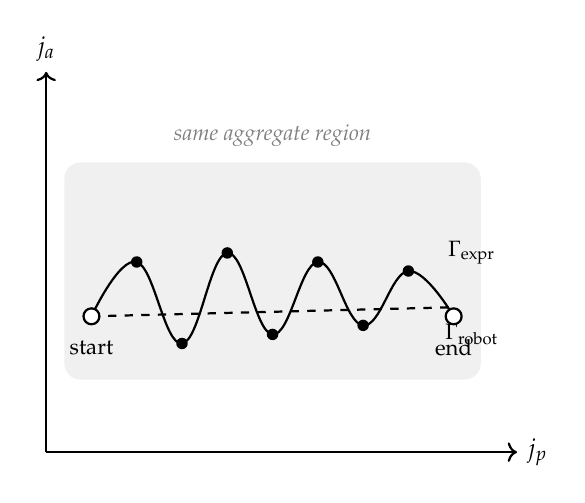
\begin{tikzpicture}[
    scale=1.15,
    axis/.style={->, thick},
    every node/.style={font=\small}
]
\draw[axis] (0,0) -- (5.2,0) node[right] {$j_p$};
\draw[axis] (0,0) -- (0,4.2) node[above] {$j_a$};

% Shaded region showing shared aggregate statistics
\fill[gray!12, rounded corners=6pt] (0.2,0.8) rectangle (4.8,3.2);
\node[font=\footnotesize\itshape, gray] at (2.5,3.5) {same aggregate region};

% Robotic trajectory — near-linear
\draw[thick, dashed]
    (0.5,1.5) -- (4.5,1.6);
\node[font=\footnotesize] at (4.7,1.3) {$\Gamma_{\mathrm{robot}}$};

% Expressive trajectory — coherent oscillation
\draw[thick]
    plot[smooth, tension=0.7] coordinates {
        (0.5,1.5)
        (1.0,2.1)
        (1.5,1.2)
        (2.0,2.2)
        (2.5,1.3)
        (3.0,2.1)
        (3.5,1.4)
        (4.0,2.0)
        (4.5,1.5)
    };
\node[font=\footnotesize] at (4.7,2.2) {$\Gamma_{\mathrm{expr}}$};

% Packet sample dots on expressive trajectory
\foreach \coord in {
    (0.5,1.5),(1.0,2.1),(1.5,1.2),(2.0,2.2),
    (2.5,1.3),(3.0,2.1),(3.5,1.4),(4.0,2.0),(4.5,1.5)
} { \fill \coord circle (1.8pt); }

% Start/end markers
\draw[fill=white, thick] (0.5,1.5) circle (2.5pt);
\draw[fill=white, thick] (4.5,1.5) circle (2.5pt);

\node[font=\footnotesize] at (0.5,1.15) {start};
\node[font=\footnotesize] at (4.5,1.15) {end};
\end{tikzpicture}
\caption{Two utterances of the same word occupy the same aggregate region of prosodic space (shaded) but differ in trajectory geometry. The robotic signal (dashed) follows a near-linear path; the expressive signal (solid) exhibits structured oscillation in the jitter dimensions, with dots indicating individual salience packet samples. Trajectory curvature and expressive coherence $\chi$ distinguish the two signals; aggregate statistics alone do not.}
\label{fig:trajectory_geometry}
\end{figure}

\begin{figure}[h]
\centering
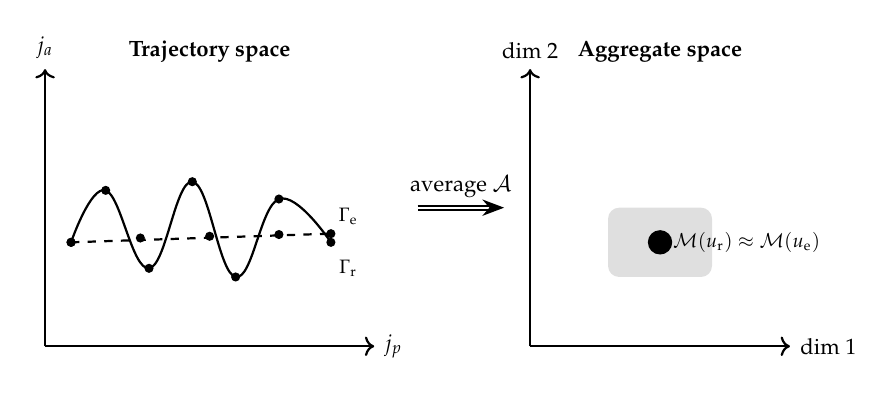
\begin{tikzpicture}[
    scale=1.1,
    every node/.style={font=\small},
    arr/.style={-{Stealth}, thick}
]
% Left panel: trajectory space
\begin{scope}[xshift=0cm]
\draw[->, thick] (0,0) -- (3.8,0) node[right, font=\footnotesize] {$j_p$};
\draw[->, thick] (0,0) -- (0,3.2) node[above, font=\footnotesize] {$j_a$};
\node[font=\footnotesize\bfseries] at (1.9,3.4) {Trajectory space};

% Robotic path
\draw[thick, dashed] (0.3,1.2) -- (3.3,1.3);
\foreach \coord in {(0.3,1.2),(1.1,1.25),(1.9,1.27),(2.7,1.29),(3.3,1.3)}
    { \fill \coord circle (1.5pt); }

% Expressive path
\draw[thick] plot[smooth, tension=0.7] coordinates
    {(0.3,1.2)(0.7,1.8)(1.2,0.9)(1.7,1.9)(2.2,0.8)(2.7,1.7)(3.3,1.2)};
\foreach \coord in {(0.3,1.2),(0.7,1.8),(1.2,0.9),(1.7,1.9),(2.2,0.8),(2.7,1.7),(3.3,1.2)}
    { \fill \coord circle (1.5pt); }

\node[font=\scriptsize] at (3.5,0.9) {$\Gamma_{\mathrm{r}}$};
\node[font=\scriptsize] at (3.5,1.5) {$\Gamma_{\mathrm{e}}$};
\end{scope}

% Arrow
\draw[arr, double] (4.3,1.6) -- node[above, font=\footnotesize]{average $\mathcal{A}$} (5.3,1.6);

% Right panel: embedding / aggregate space
\begin{scope}[xshift=5.6cm]
\draw[->, thick] (0,0) -- (3.0,0) node[right, font=\footnotesize] {dim 1};
\draw[->, thick] (0,0) -- (0,3.2) node[above, font=\footnotesize] {dim 2};
\node[font=\footnotesize\bfseries] at (1.5,3.4) {Aggregate space};

% Both collapse to same region
\fill[gray!25, rounded corners=4pt] (0.9,0.8) rectangle (2.1,1.6);
\fill (1.5,1.2) circle (4pt);
\node[font=\scriptsize] at (2.5,1.2) {$\mathcal{M}(u_{\mathrm{r}}) \approx \mathcal{M}(u_{\mathrm{e}})$};
\end{scope}
\end{tikzpicture}
\caption{Failure mode of aggregate-only analysis. In trajectory space (left), the robotic path $\Gamma_{\mathrm{r}}$ (dashed) and expressive path $\Gamma_{\mathrm{e}}$ (solid) are geometrically distinct. After averaging via $\mathcal{A}$ (right), both collapse to the same region of aggregate feature space, making them indistinguishable. Expressive coherence $\chi$ and trajectory-level DTW are required to recover the distinction.}
\label{fig:embedding_collapse}
\end{figure}


\section{Triangular Equivalence}

The full equivalence \eqref{eq:fullequiv} has a natural geometric form. The three trajectory representations---audio, memory, and text---are not linearly ordered but mutually projectable: any two can be converted to the third via the operators defined in the preceding sections. This mutual projectability is represented in Figure~\ref{fig:triangle}.

\begin{figure}[h]
\centering
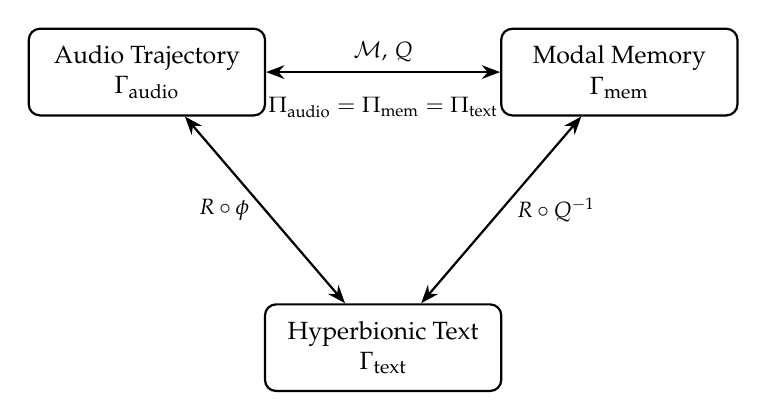
\begin{tikzpicture}[
    every node/.style={font=\small},
    box/.style={rectangle, draw, thick, rounded corners, align=center,
                minimum width=3.0cm, minimum height=1.1cm, fill=white},
    arr/.style={{Stealth}-{Stealth}, thick},
    label/.style={font=\footnotesize\itshape}
]
\node[box] (audio) at (0, 0)    {Audio Trajectory\\$\Gamma_{\mathrm{audio}}$};
\node[box] (mem)   at (6, 0)    {Modal Memory\\$\Gamma_{\mathrm{mem}}$};
\node[box] (text)  at (3, -3.5) {Hyperbionic Text\\$\Gamma_{\mathrm{text}}$};

\draw[arr] (audio) -- node[label, above]{$\mathcal{M},\,Q$} (mem);
\draw[arr] (audio) -- node[label, left, xshift=-2pt]{$R \circ \phi$} (text);
\draw[arr] (mem)   -- node[label, right, xshift=2pt]{$R \circ Q^{-1}$} (text);

\node[font=\footnotesize, align=center] at (3,-0.45)
    {$\Pi_{\mathrm{audio}} = \Pi_{\mathrm{mem}} = \Pi_{\mathrm{text}}$};
\end{tikzpicture}
\caption{Triangular equivalence of the three trajectory representations. Each vertex is a representation of the same prosodic invariant structure in a different medium. The double-headed arrows indicate structure-preserving projections in both directions. The central identity states that all three projection operators extract the same invariants from their respective media.}
\label{fig:triangle}
\end{figure}

\begin{definition}[Prosodic Invariant Field]
The \emph{prosodic invariant field} is the equivalence class of all representations---audio, modal, typographic---that preserve the projection operator $\Pi$. Formally, it is the fiber over $\Pi$ in the bundle of signal representations over the shared parameter space.
\end{definition}

The three vertices of the triangle are sections of this field over different media. The equivalence \eqref{eq:fullequiv} holds conditionally: $\Pi_{\mathrm{audio}}(u) = \Pi_{\mathrm{mem}}(Z) = \Pi_{\mathrm{text}}(R(g,p))$ if and only if the operators $R$ and $Q$ are \emph{admissible} in the sense of being invariant-preserving (no distinctions present in the parameter space are collapsed) and non-collapsing (no distinctions absent from the parameter space are introduced). This makes triangular equivalence a design criterion testable by inspection of the rendering and quantization maps.

The three sides of the triangle correspond to three distinct operations. The top edge is the Marine--MEM$|$8 chain: acoustic measurement $\mathcal{M}$ followed by fixed-point quantization $Q$, converting audio trajectories into modal lattice coordinates. The left edge is the rendering chain: the projection $\phi$ from packet space to prosodic parameter space followed by the Hyperbionic rendering operator $R$, converting audio trajectories directly into visual typography. The right edge is the reconstruction chain $R \circ Q^{-1}$: reading a Hyperbionic rendering back through the inverse quantization to recover a prosodic vector, and then synthesizing an audio trajectory consistent with that vector.

The central identity $\Pi_{\mathrm{audio}} = \Pi_{\mathrm{mem}} = \Pi_{\mathrm{text}}$ is the claim that all three projection operators extract the same invariant structure. This is not a tautology: it is a constraint on the design of the rendering operator $R$ and the quantization operator $Q$, requiring that neither introduces distinctions not present in the prosodic parameter space and neither collapses distinctions that the other preserves. A rendering operator that maps two distinct prosodic vectors to the same visual output violates the constraint; so does a quantization scheme that conflates vectors that the rendering operator distinguishes. The triangular equivalence is therefore a testable design criterion, not merely a philosophical claim.


\section{Conclusion}

The preceding sections have developed a single invariant structure expressed across three media: acoustic signal, geometric trajectory, and visual typography. Hyperbionic Reading is not an enhancement of text, and the three representations are not projections from a richer object to progressively poorer ones. \hyperstrong{They are coordinate charts on a shared invariant field}---different parameterizations of the same underlying prosodic structure, each complete within its medium and mutually convertible through the operators $\mathcal{M}$, $Q$, and $R$. The boundary between writing and signal processing is not extended but removed: both are coordinate representations of the same invariant field. The argument developed in this essay has three levels.

At the representational level, acoustic waveforms, MEM$|$8 modal coordinates, and Hyperbionic typographic renderings are equivalent as parameterized projections of a shared prosodic parameter space. The equivalence is formalized by the commuting chain $\mathcal{M} \to Q \to R$ and the projection operators $\Pi_{\mathrm{audio}}$, $\Pi_{\mathrm{mem}}$, $\Pi_{\mathrm{text}}$.

At the operational level, higher-dimensional acoustic features---delay and reverberation---admit precise typographic operators: delay becomes spatial displacement, reverberation becomes convolutional diffusion. The time-to-space correspondence is not an analogy; it is an isomorphism between the parameter spaces of acoustic signal processing and typographic rendering.

At the dynamical level, extending the framework to continuous speech treats spoken words as trajectories through modal space rather than as static feature vectors. The resulting trajectory resonance architecture for speech recognition is wave-native: it stores words as paths, compares paths by a time-warped coherence functional, and recognizes by resonant collapse rather than classification. This unifies acoustic analysis, modal storage, Hyperbionic rendering, and speech recognition as instances of trajectory reconstruction across modalities.

The central consequence is the inclusion~\eqref{eq:inclusion}: plain text, parameterized text, and the full multimodal resonance field form a strict hierarchy of representational richness. Moving up this hierarchy does not add decoration to language; it recovers dimensions of communicative structure that plain transcription discards. Typography, extended into the Hyperbionic system, becomes a genuine carrier of prosodic information, and the boundary between writing and signal processing dissolves.

\begin{thebibliography}{9}

\bibitem{Tulving1982}
Tulving, E. (1982).
Synergistic ecphory in recall and recognition.
\textit{Canadian Journal of Psychology / Revue canadienne de psychologie}, 36(2), 130--147.
\url{https://doi.org/10.1037/h0080641}

\bibitem{Cabral2023}
Cabral, J., Fernandes, F.\,F., \& Shemesh, N. (2023).
Intrinsic macroscale oscillatory modes driving long range functional connectivity in female rat brains detected by ultrafast fMRI.
\textit{Nature Communications}, 14, 375.
\url{https://doi.org/10.1038/s41467-023-36025-x}

\bibitem{Marder1996}
Marder, E., \& Calabrese, R.\,L. (1996).
Principles of rhythmic motor pattern generation.
\textit{Physiological Reviews}, 76(3), 687--717.

\bibitem{Needham1997}
Needham, T. (1997).
\textit{Visual Complex Analysis}.
Oxford University Press.

\end{thebibliography}

\end{document}

